% this file is called up by thesis.tex
% content in this file will be fed into the main document

% --------- begin appendices --------- %

\begin{appendices}

%: ----------------------- paths to graphics ------------------------

\graphicspath{{9_appendix/images/}}

%: ----------------------- contents from here ------------------------


% --------- ngram analysis --------- %

\chapter{n-gram frequency analysis}
\label{appendix:ngramanalysis}

During our analysis of the Public BI benchmark we noticed several \verb|VARCHAR| columns containing strings that are concatenations of data from different distributions. These columns can be stored more efficiently in separate subcolumns, in order to allow independent compression of their constituent parts. We approached this problem with the \nameref{subsec:pd:charsetsplit} pattern detector (\ref{subsec:pd:charsetsplit}) and obtained good results, but we did not cover all the variations of such columns. Table~\ref{tab:appendix:ngramanalysis:table1} shows two samples of data from columns that have this property but we did not cover.

% \begin{table}[h]
% \centering

% \caption{Eixo\_1 data sample}
% \label{tab:appendix:ngramanalysis:table1}
% \end{table}

\begin{table}[h]
% \centering
\small
\begin{minipage}{.4\linewidth}
% \centering
\begin{tabular}{@{}l@{}}
\toprule
ds\_email                             \\ \midrule
\verb|ic.caetano@hotmail.com|        \\
\verb|arnaldo2moraes@yahoo.com.br|   \\
\verb|s_heique266@yahoo.com.br|      \\
\verb|silasvkj@hotmail.com|          \\
\verb|leonel_noga@hotmail.com|       \\
\verb|alexelidi@yahoo.com.br|        \\
\verb|jdcn488@hotmail.com|           \\
\verb|elton.t.santos@gmail.com|      \\
\verb|kassiosgoda@hotmail.com|       \\
\verb|valdireneandrade1@hotmail.com| \\
\verb|diego.shynomory@gmail.com|     \\
\verb|fer-ars@hotmail.com|           \\
\verb|rosilda_limactba@hotmail.com|  \\
\verb|utfpraasma@hotmail.com|        \\ \bottomrule
\end{tabular}
% \caption*{ds\_email}
\end{minipage}%
\begin{minipage}{.6\linewidth}
% \centering
\begin{tabular}{@{}l@{}}
\toprule
ds\_tipo\_beneficiario                                   \\ \midrule
\verb|Outro: especificar - bolsa formação estudante|     \\
\verb|Outro: especificar - Programa Nacional de [...]|   \\
\verb|Outro: especificar - cadastro unico|               \\
\verb|Outro: especificar - aluno ensino Médio|           \\
\verb|Beneficiário de [...] - Beneficiário de [...]|     \\
\verb|Outro: especificar - aluno da rede publica|        \\
\verb|Outro: especificar - aluno escola publica|         \\
\verb|Atendimento prioritário - Atendimento prioritário| \\
\verb|Outro: especificar - Outro: especificar|           \\
\verb|Outro: especificar - Outro: especificar|           \\
\verb|Outro: especificar - ESTUDANTE REDE PUBLICA|       \\
\verb|Outro: especificar - nao é perfil cadunico|        \\
\verb|Outro: especificar - CADÚNICO|                     \\
\verb|Outro: especificar - possui renda inferior [...]|  \\ \bottomrule
\end{tabular}
% \caption*{ds\_tipo\_beneficiario}
\end{minipage}
\caption{Eixo\_1 data samples}
\label{tab:appendix:ngramanalysis:table1}
\end{table}


Both columns are composed of two parts: one with high repetition factor---which can benefit from compression---and one rather unique---which cannot. They are separated by a delimiter character: \verb|'@'|, respectively \verb|'-'|. While the \nameref{subsec:pd:charsetsplit} could cover these columns with a delimiter character set (e.g. \verb|[@-]|), there are also cases with no explicit separator character but other structures instead (e.g. fixed number of characters from the start of each string). 

To cover all cases in a more generic way, we tried to develop a different approach based on n-gram frequencies. We represented each string in a different way, such that we can identify its constituent substrings more easily, as follows: 1) we computed the frequencies of all 3-grams based on their number of occurrences on the entire column; 2) we replaced each character in each string with the frequency of the 3-gram starting at the position of the character. The results are presented in Figures \ref{fig:appendix:ngramanalysis:ngram_1} and \ref{fig:appendix:ngramanalysis:ngram_2}.

\begin{figure}[h]
  \centering
  \makebox[\textwidth][c]{
    \includesvg[width=0.95\linewidth]{ngram-col_28.svg}
  }
  \caption{\textit{ds\_email} 3-gram frequencies}
  \label{fig:appendix:ngramanalysis:ngram_1}
\end{figure}

\begin{figure}[h]
  \centering
  \makebox[\textwidth][c]{
    \includesvg[width=0.95\linewidth]{ngram-col_30.svg}
  }
  \caption{\textit{ds\_tipo\_beneficiario} 3-gram frequencies}
  \label{fig:appendix:ngramanalysis:ngram_2}
\end{figure}

The figures show the frequency of the 3-grams in the strings in the two columns presented above (larger samples than in the example). The Y axis represents each string on the column and the X axis contains the positions of the characters in the strings. The colors represent the frequencies: white = high frequency, red = low frequency. Black is used as padding for shorter strings. Figure~\ref{fig:appendix:ngramanalysis:ngram_1} shows the results for the \textit{ds\_email} column. We notice how all the emails start with low frequencies (the local/username part) and end with high frequencies (the domain part). Moreover, we can also observe the different components of the domain: we have the top level domains with the highest frequencies (e.g. \verb|.com|, \verb|.br|, etc.), followed by the subdomains (e.g. \verb|gmail|, \verb|hotmail|, etc.). Even more, the word \verb|"mail"| is also representative in itself, since it is common for most email subdomains. Figure~\ref{fig:appendix:ngramanalysis:ngram_2} shows the results for the \textit{ds\_tipo\_beneficiario} column. It is clear how the majority of the strings start with the frequent substring \verb|"Outro: especificar"| and end in a low frequency substring.

The 3-gram frequency representation emphasizes the constituent subparts in which a column should be split in order to enable independent compression. The goal is to automatically find the split points, which is not a trivial task. The approach that we propose relies on the fact that we can view each string as a series of numbers (3-gram frequencies). The series contain edges and plateaus. An edge is a significant increase or decrease in frequency. After identifying the edges in each string, we need to find the common edges amongst the majority of the strings. A common edge is an edge that can be identified either by the same character (e.g. the \verb|'@'| delimiter) or by the same absolute position in all the strings. Once we found the common edges, we define the split points based on the character or position. During compression, we split each string according to these identifiers and mark as exception the values that cannot be split.

Due to time constraints, we decided not to proceed with the implementation and evaluation of this approach and leave it for future work.

\chapter{Column correlation graphs}
\label{appendix:corrgraphs}

The figures below show two examples of \nameref{subsec:pd:columncorrelation} graphs as defined in \ref{subsubsec:ps:correlation}. Figure~\ref{fig:appendix:corrgraphs:yale} shows a common correlation graph resulted from Configuration B (\ref{sec:eval:expsetup}) after applying the \nameref{subsec:pd:columncorrelation} pattern detector (\ref{subsec:pd:columncorrelation}) on the leaf columns of the tree produced by the \nameref{sub:learning:recursiveexhaustive} algorithm (\ref{sub:learning:recursiveexhaustive}) in \textit{Stage-1} (table: \textit{YaleLanguages\_1}).
Figure~\ref{fig:appendix:corrgraphs:generico} shows a highly complex correlation graph, resulted from Configuration A (\ref{sec:eval:expsetup}) (table: \textit{Generico\_1}). Both configurations resulted in graphs of similar complexities for the same tables. An important note is that these correlations are not directly between the logical columns, but between subcolumns resulted after decomposing them and separating the values into different subsets and exceptions as well. As we see in the figures, this process creates many correlation opportunities---and most of them could not be exploited on the original representation of the data.

Columns with high indegree can be determined by many other columns. This happens to columns that are (almost) constant and---in our case in particular---to exception columns with very high null ratios. The explanation is that, if a column has the same constant value (e.g. \verb|null|), any other column can determine it since all its values will map to the constant value. Columns with high outdegree can determine many other columns. This happens to columns with very low repetition factor (i.e. rather unique), since there is a perfect mapping between a unique column and any other column. However, this does not happen in our case, since we only use \nameref{subsec:pd:columncorrelation} on \nameref{subsec:pd:dict} compressible columns. Besides these special cases of nearly constant or unique columns, high degrees result from actual correlations between (sub)columns created by the learning algorithms.

% The correlation coefficients are computed as described in \ref{todo}. Recall that column correlation only applies on Dict represented columns and therefore the graph only contains these columns.

\begin{sidewaysfigure}[h]
  \centering
  \makebox[\textwidth][c]{
    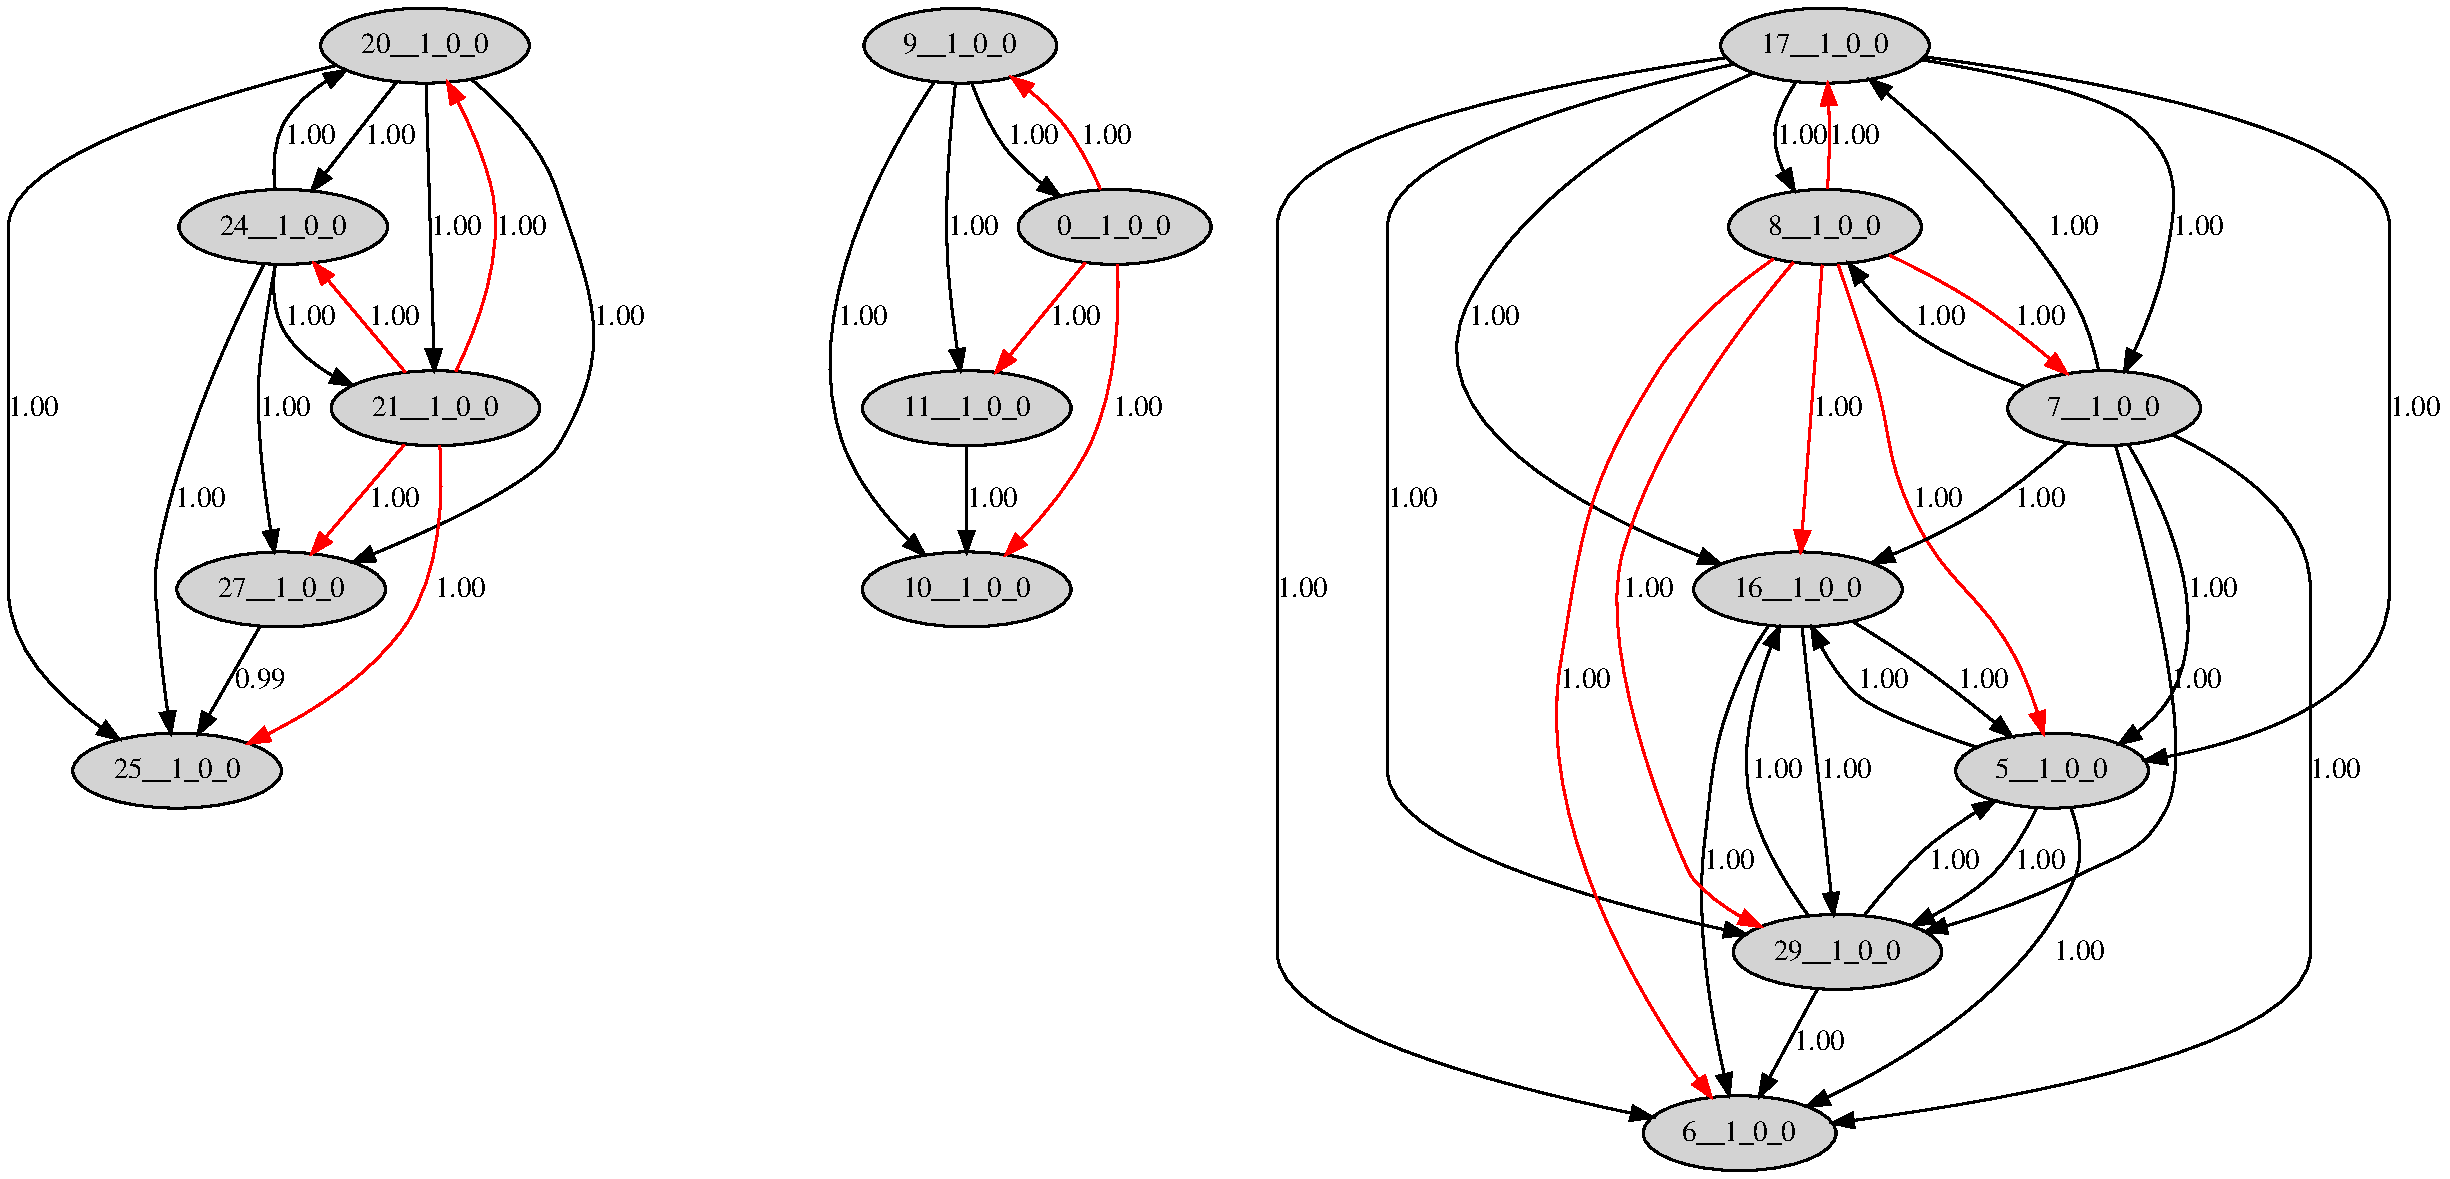
\includegraphics[width=0.88\linewidth]{YaleLanguages_1-s_1_l_0-graph.pdf}
  }
  \caption{\textit{YaleLanguages\_1} correlation graph}
  \label{fig:appendix:corrgraphs:yale}
\end{sidewaysfigure}

\begin{sidewaysfigure}[h]
  \centering
  \makebox[\textwidth][c]{
    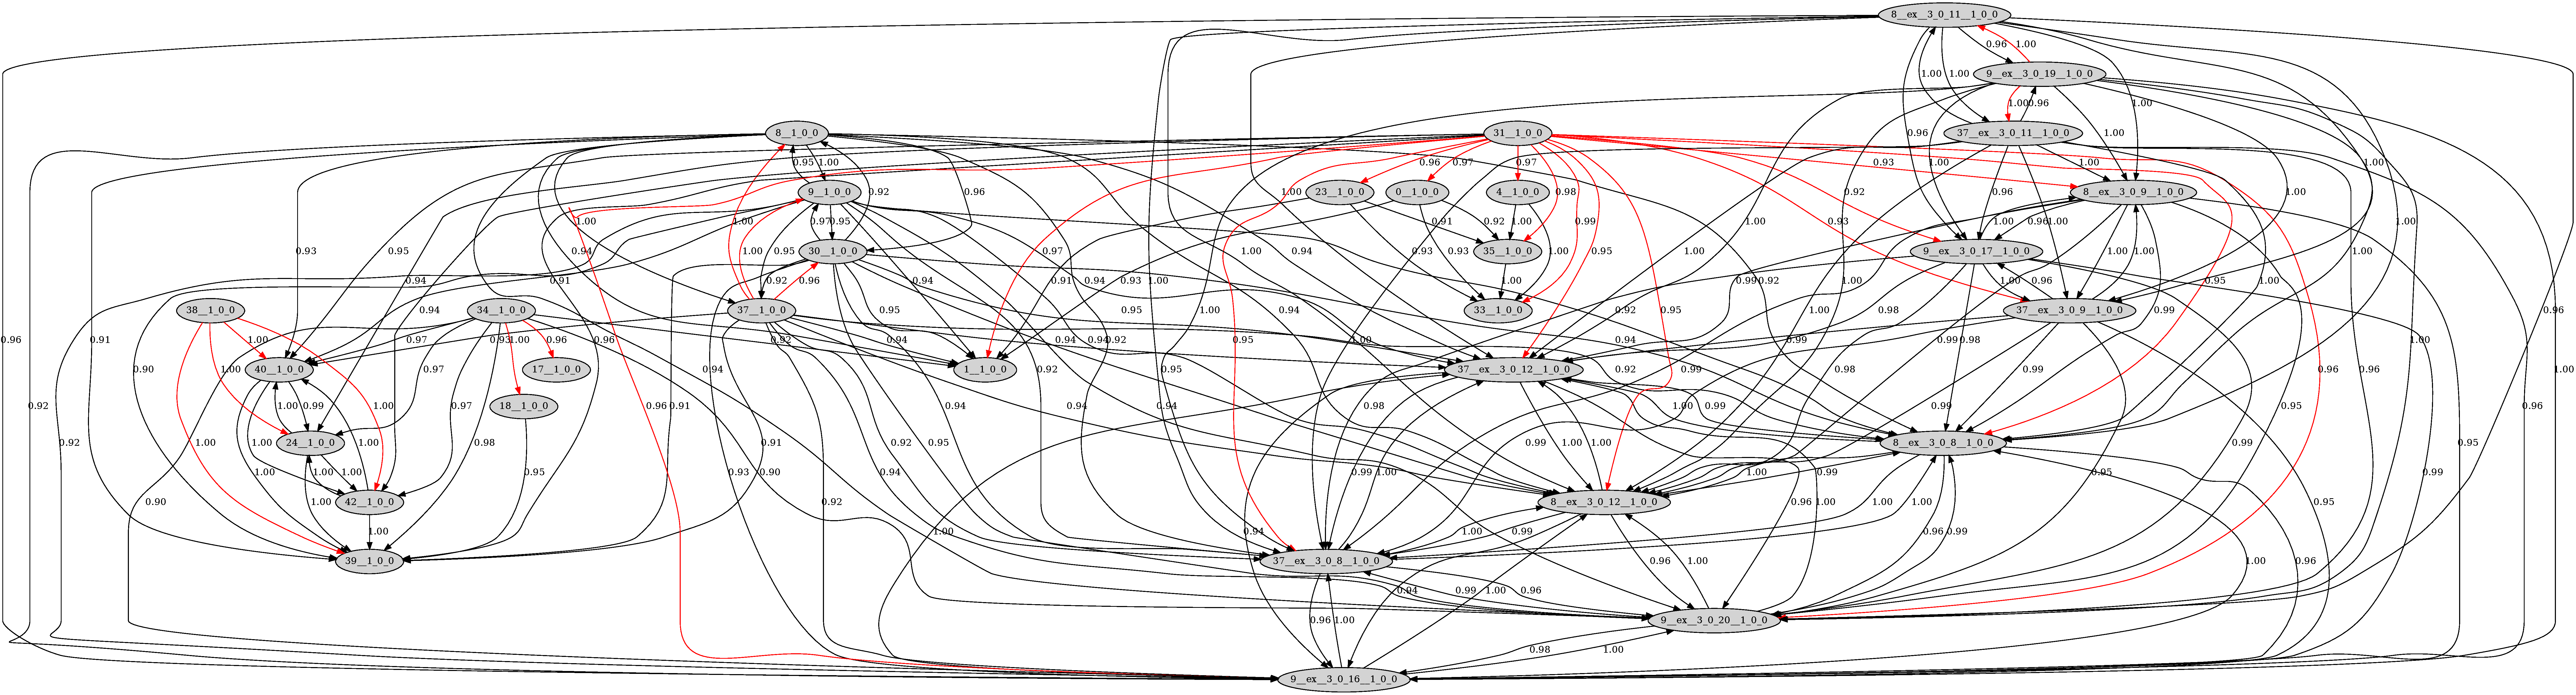
\includegraphics[width=1.08\linewidth]{Generico_1-corr-s_1_l_0-graph.pdf}
  }
  \caption{\textit{Generico\_1} correlation graph}
  \label{fig:appendix:corrgraphs:generico}
\end{sidewaysfigure}


% --------- notes --------- %

\iffalse
- interesting results:
  - correlation graphs \& heatmaps
  - pattern distribution
  - n-gram analysis
  - other plots that you already have
- concrete examples of whitebox representation of interesting columns (similar to the ones in presentation); with calculation of compression ratio, etc.
\fi

\iffalse
To better understand the impact of \textit{whitebox compression} and how it affects the compression ratio we selected \verb|todo| representative tables and analyzed their compression trees and size components. TODO-1: analyze 2-3 tables

analyze:
YaleLanguages - very good with both vw and wc, but small
Generico - large, decent with vw, significantly good with wb
Redfin1\_1 - not good overall, but good in used -> lack of compression opportunities
RealEstate2\_1 - not good with used either
\fi


% --------- end appendices --------- %

\end{appendices}

% ---------------------------------------------------------------------------
%: ----------------------- end of thesis sub-document ------------------------
% ---------------------------------------------------------------------------

